\documentclass[twocolumn, 10pt]{article}


\usepackage[
	filename=false, 
	allfiguresdraft=false
]{draftfigure}


% --- Page Layout --- %

\usepackage[utf8]{inputenc}
\usepackage{xcolor}
\usepackage{geometry}
\geometry{
	a4paper,
	left=20.0mm,
	right=20.0mm,
	top=20.0mm,
	bottom=22.0mm,
	columnsep=5.0mm,
	headsep=6.5mm,
	footskip=12.5mm
}
\usepackage[aux]{rerunfilecheck}
\usepackage{dblfloatfix}


% --- Modern Font Setup --- %

\usepackage{fontspec}
\usepackage{unicode-math}
\setmainfont{TeX Gyre Termes}
\setmathfont{TeX Gyre Termes Math}


% --- Math Symbols --- %

\usepackage{amsmath}
\usepackage{mathtools}


% --- Units --- %

\usepackage[
	locale=US,
	per-mode = power,
	exponent-mode = input,
	print-unity-mantissa = false,
	range-units = single
]{siunitx}

\DeclareSIUnit{\year}{yr}
\DeclareSIUnit{\erg}{erg}
\DeclareSIUnit{\parsec}{pc}
\DeclareSIUnit{\solarmass}{\ensuremath{M_\odot}}


% --- Aesthetic Improvements --- %

\usepackage{graphicx}
\usepackage{booktabs}
\usepackage{microtype}
\usepackage[autostyle]{csquotes}


% --- Float Improvements --- %

\usepackage{float}
\floatplacement{figure}{htbp}
\floatplacement{table}{htbp}

\usepackage[
	section,
	below,
]{placeins}


% --- Abstract Adjustments --- %

\usepackage{abstract}
\renewcommand{\abstracttextfont}{\small}
\setlength{\absleftindent}{0pt}
\setlength{\absrightindent}{0pt}
\setlength{\abstitleskip}{0.25\baselineskip}
\AfterEndEnvironment{abstract}{\vspace{1.5\baselineskip}}


% --- Section Styling --- %

\usepackage{titlesec}
\titleformat{\section}{\normalfont\large\bfseries}{\thesection}{1ex}{}
\titleformat{\subsection}{\normalfont\normalsize\bfseries}{\thesubsection}{1ex}{}


% --- Caption Styling --- %
\usepackage[
	labelfont=bf,
	font=small,
]{caption}
\usepackage{subcaption}

\captionsetup[figure]{width=0.9\columnwidth}
\captionsetup[figure*]{width=0.9\textwidth}

% --- Header & Footer --- %

\usepackage{fancyhdr}
\pagestyle{fancy}

\fancyhf{}
\renewcommand{\headrulewidth}{0pt}
\fancyfoot[C]{\itshape\thepage}

\fancypagestyle{plain}{
  \fancyhf{}
  \fancyfoot[C]{\itshape\thepage}
  \renewcommand{\headrulewidth}{0pt}
}


% --- Citation Setup --- %

\usepackage[american]{babel}

\usepackage[
	colorlinks=true, 
	linkcolor=black,      
	citecolor=black,      
	urlcolor=black        
]{hyperref}

\usepackage[noabbrev]{cleveref}
\newcommand{\bcref}[1]{\textbf{\cref{#1}}}
\newcommand{\bCref}[1]{\textbf{\Cref{#1}}}

\usepackage[
	backend=biber,
	style=authoryear,
	giveninits=true,   
	maxnames=2,        
	minnames=1,
	uniquename=false,
	uniquelist=false
]{biblatex}

\DeclareNameAlias{author}{family-given} 
\DeclareDelimFormat{multinamedelim}{\addspace\&\addspace}
\DeclareDelimFormat{finalnamedelim}{\addspace\&\addspace}
\DefineBibliographyStrings{english}{andothers={et al.}} 

\DeclareFieldFormat{labeldate:extrayear}{}

\DeclareCiteCommand{\cite}[\mkbibparens]
	{\usebibmacro{prenote}}%
	{\usebibmacro{citeindex}%
	 \printtext[bibhyperref]{%
	 	\printnames{labelname}%
	 	\setunit{\addspace}%
	 	\printfield{labelyear}%
	 	\printfield{extrayear}%
	 }%
	}%
	{\multicitedelim}%
	{\usebibmacro{postnote}}%

\DeclareDelimFormat{multicitedelim}{\addcomma\addspace}

\DeclareFieldFormat[article,periodical]{journaltitle}{\textit{#1}}

\DeclareFieldFormat[article]{title}{}
\DeclareFieldFormat[book]{title}{}

\AtEveryBibitem{%
	\clearfield{volume}%
	\clearfield{number}%
	\clearfield{pages}%
	\clearfield{note}%
	\clearfield{location}%
	\clearfield{address}%
}

\renewcommand{\finentrypunct}{}

\DeclareBibliographyDriver{article}{%
	\usebibmacro{bibindex}%
	\usebibmacro{begentry}%
	\iffieldundef{doi}
		{\iffieldundef{url}
			{\printnames{author}\setunit{\addspace}%
			 \usebibmacro{journal}\setunit{\addspace}%
			 \printtext{\mkbibparens{\printfield{labelyear}\printfield{extrayear}}}}%
			{\href{\thefield{url}}{%
				\printnames{author}\setunit{\addspace}%
				\usebibmacro{journal}\setunit{\addspace}%
				\printtext{\mkbibparens{\printfield{labelyear}\printfield{extrayear}}}}}}
		{\href{https://doi.org/\thefield{doi}}{%
			\printnames{author}\setunit{\addspace}%
			\usebibmacro{journal}\setunit{\addspace}%
			\printtext{\mkbibparens{\printfield{labelyear}\printfield{extrayear}}}}}%
	\usebibmacro{finentry}%
}

\addbibresource{source.bib}


% --- Paragraph Skip --- %

\usepackage{parskip}
\setlength{\parindent}{0pt}
\setlength{\parskip}{0.4\baselineskip plus 2pt minus 2pt}


% --- Linted Code --- %

\usepackage{varwidth}
\usepackage{listings}
\usepackage{accsupp}

\newcommand{\noncopynumber}[1]{%
     \BeginAccSupp{ActualText={}}#1\EndAccSupp{}%
}

\definecolor{firebrick}{RGB}{178, 34, 34}     
\definecolor{goldenrod}{RGB}{218, 165, 32}    
\definecolor{olivedrab}{RGB}{107, 142, 35}    
\definecolor{steelblue}{RGB}{70, 130, 180}    
\definecolor{rebeccapurple}{RGB}{102, 51, 153}

\definecolor{lightergray}{RGB}{250, 250, 250} 
\definecolor{lightishgray}{RGB}{180, 180, 180}

\lstset{
	language=SQL,                          
	backgroundcolor=\color{lightergray},   
	basicstyle=\ttfamily\footnotesize\color{black},
	identifierstyle=\color{black},
	keywordstyle=\color{steelblue}\bfseries, 
	stringstyle=\color{goldenrod},        
	morekeywords=[2]{TOP, APPLY},
	keywordstyle=[2]{\color{firebrick}\bfseries},
	numberstyle=\tiny\color{lightishgray}\noncopynumber, 
	numbers=left,                          
	numbersep=8pt,                         
	breaklines=true,                       
	breakatwhitespace=false,               
	showstringspaces=false,                
	keepspaces=true,
	frame=single,                          
	rulecolor=\color{black},
	tabsize=4,                             
	keywordsprefix=,
	literate=*
		{=}{{{\color{rebeccapurple}=}}}1
		{!=}{{{\color{rebeccapurple}!=}}}2
		{<}{{{\color{rebeccapurple}<}}}1
		{>}{{{\color{rebeccapurple}>}}}1
		{+}{{{\color{rebeccapurple}+}}}1
		{-}{{{\color{rebeccapurple}-}}}1
		{*}{{{\color{rebeccapurple}*}}}1
		{:}{{{\color{rebeccapurple}:}}}1
		{10000}{{{\color{olivedrab}10000}}}5
		{\ 1\ }{{{\ \color{olivedrab}1\ }}}3
		{\ 3}{{{\ \color{olivedrab}3}}}2
		{0\.35}{{{\color{olivedrab}0.35}}}4
		{\ 0\.0}{{{\ \color{olivedrab}0.0}}}4
		{5\.0}{{{\color{olivedrab}5.0}}}3
		{2\.355}{{{\color{olivedrab}2.355}}}5
		{\ 500}{{{\ \color{olivedrab}500}}}4
}


% --- Dummy Text --- %

\usepackage{lipsum}


% --- Writing Lengths --- %

\AtEndDocument{
	\directlua{
		local factor = 65536 * 72.27
		
		local tw = math.floor((tex.getdimen("textwidth") / factor) * 100 + 0.5) / 100
		local cw = math.floor((tex.getdimen("columnwidth") / factor) * 100 + 0.5) / 100
		local cs = math.floor((tex.getdimen("columnsep") / factor) * 100 + 0.5) / 100
		local lw = math.floor((tex.getdimen("linewidth") / factor) * 100 + 0.5) / 100
		
		texio.write_nl("===================================================")
		texio.write_nl("CURRENT LAYOUT:")
		texio.write_nl("Textwidth:  " .. tw .. " in")
		texio.write_nl("Columnwidth: " .. cw .. " in")
		texio.write_nl("Columnsep:   " .. cs .. " in")
		texio.write_nl("Linewidth:   " .. lw .. " in")
		texio.write_nl("===================================================")
		io.flush()
	}
}



% --- Title --- %

\title{\textbf{Characterization of Galaxies via Optical and Infrared Surveys}}%


% --- Author --- %

\author{Fritz Ali Agildere%
		\vspace{-0.5ex}\\\small\href{mailto:fritz.agildere@udo.edu}{fritz.agildere@udo.edu}%
		\\\small\textit{Department of Astronomy, Faculty of Mathematics, University of Belgrade}}%


% --- Compilation Date --- %

\date{\small \today}


% --- Header & Footer --- %

\fancyhead[C]{\textit{Characterization of Galaxies via Optical and Infrared Surveys}}
\fancyfoot[L]{\textit{\textls[9]{Introduction{\kern+4pt}to{\kern+4pt}Active{\kern+4pt}Galactic{\kern+4pt}Nuclei}}}
\fancyfoot[R]{\textit{\textls[-6]{Master{\kern+2pt}in{\kern+2pt}Astrophysics{\kern+2pt}and{\kern+2pt}Space{\kern+2pt}Science}}}

\fancypagestyle{plain}{
	\fancyhead[C]{}
	\fancyfoot[L]{\textit{\textls[9]{Introduction{\kern+4pt}to{\kern+4pt}Active{\kern+4pt}Galactic{\kern+4pt}Nuclei}}}
	\fancyfoot[R]{\textit{\textls[-6]{Master{\kern+2pt}in{\kern+2pt}Astrophysics{\kern+2pt}and{\kern+2pt}Space{\kern+2pt}Science}}}
}


% --- Custom Macros --- %

\newcommand{\dash}{\rule[0.49ex]{0.35em}{0.06em}}
\newcommand{\xray}{X\hspace{0.04em}\dash\hspace{0.11em}ray\space}
\newcommand{\xrays}{X\hspace{0.04em}\dash\hspace{0.11em}rays\space}


% --- Metadata --- %

\hypersetup{
	pdfauthor={Fritz Ali Agildere},
	pdftitle={Course Report – Fritz Agildere}
}


% --- Begin Document --- %

\begin{document}

	\twocolumn[{
		\maketitle
		\begin{abstract}
			\lipsum[1]
		\end{abstract}
	}]
	
	\begin{figure}
		\centering
		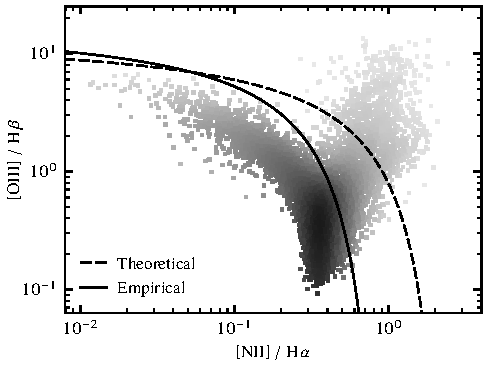
\includegraphics[width=\columnwidth, draft=false]{assets/plots/BPT_scatter.pdf}
		\caption{}
		\label{fig:BPT_scatter}
	\end{figure}
	
	\begin{figure}
		\centering
		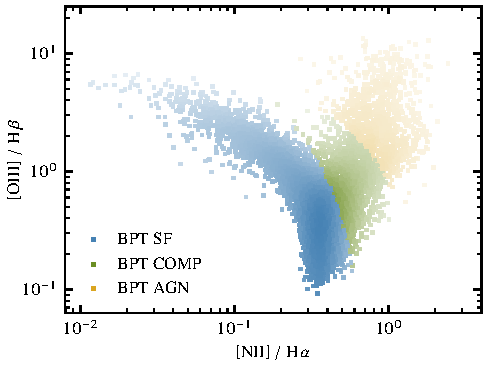
\includegraphics[width=\columnwidth, draft=false]{assets/plots/BPT_class.pdf}
		\caption{}
		\label{fig:BPT_class}
	\end{figure}
	
	\begin{figure}
		\centering
		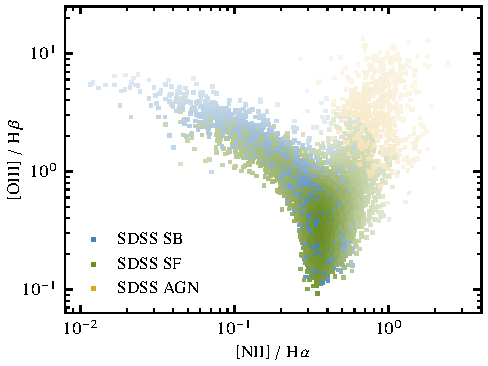
\includegraphics[width=\columnwidth, draft=false]{assets/plots/BPT_SDSS_class.pdf}
		\caption{}
		\label{fig:BPT_SDSS_class}
	\end{figure}
	
	\begin{figure}
		\centering
		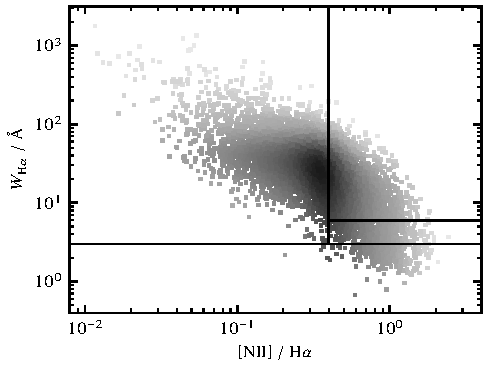
\includegraphics[width=\columnwidth, draft=false]{assets/plots/WHAN_scatter.pdf}
		\caption{}
		\label{fig:WHAN_scatter}
	\end{figure}
	
	\begin{figure}
		\centering
		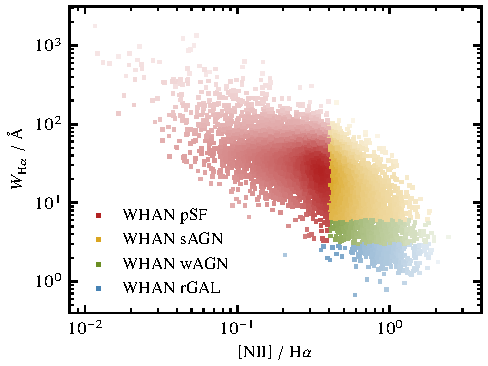
\includegraphics[width=\columnwidth, draft=false]{assets/plots/WHAN_class.pdf}
		\caption{}
		\label{fig:WHAN_class}
	\end{figure}
	
	\begin{figure}
		\centering
		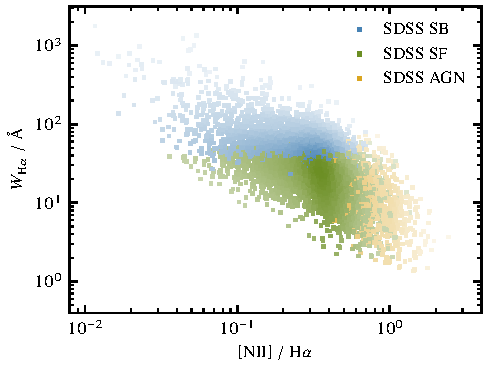
\includegraphics[width=\columnwidth, draft=false]{assets/plots/WHAN_SDSS_class.pdf}
		\caption{}
		\label{fig:WHAN_SDSS_class}
	\end{figure}

	\begin{figure}
		\centering
		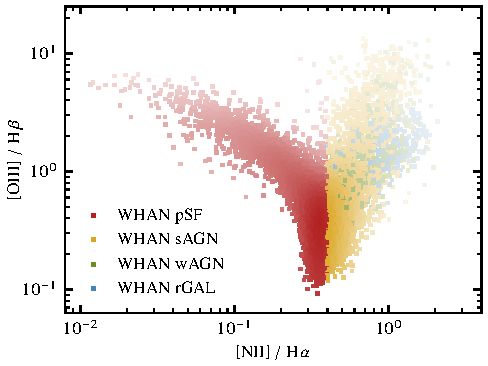
\includegraphics[width=\columnwidth, draft=false]{assets/plots/BPT_WHAN_class.pdf}
		\caption{}
		\label{fig:BPT_WHAN_class}
	\end{figure}

	\begin{figure}
		\centering
		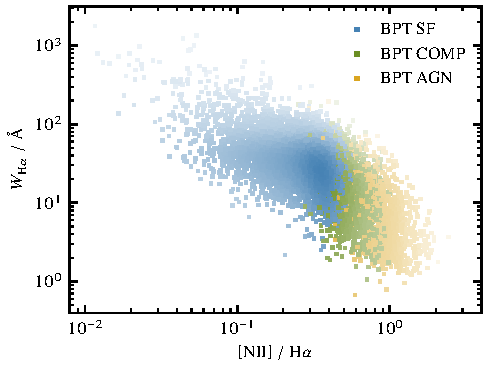
\includegraphics[width=\columnwidth, draft=false]{assets/plots/WHAN_BPT_class.pdf}
		\caption{}
		\label{fig:WHAN_BPT_class}
	\end{figure}

	\begin{figure*}[t]
		\centering
		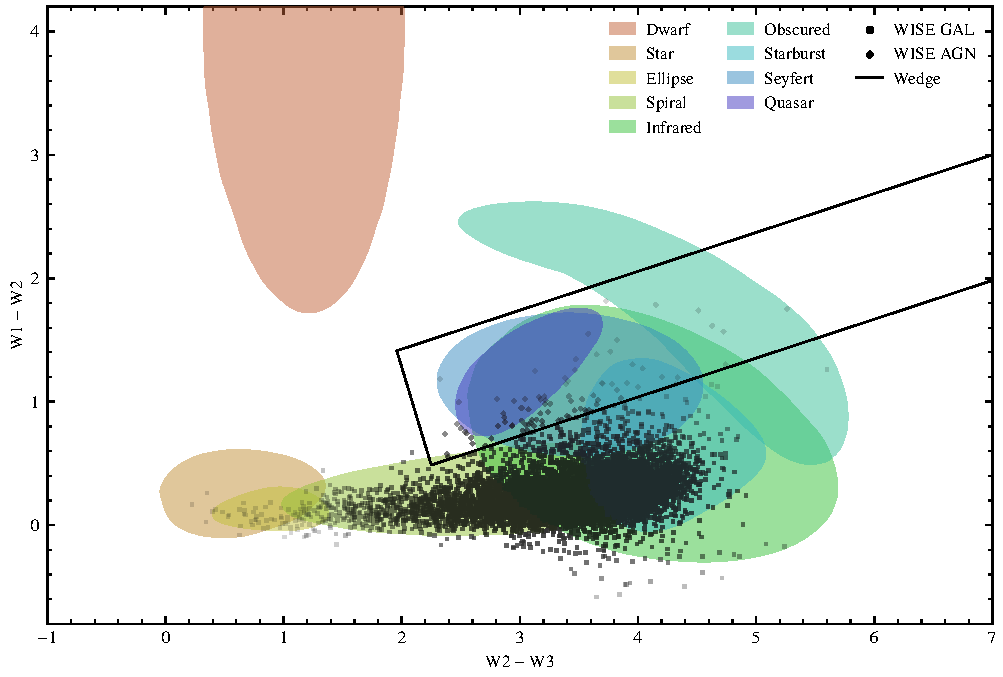
\includegraphics[width=\textwidth, draft=false]{assets/plots/WISE_overlay.pdf}
		\caption{}
		\label{fig:WISE_overlay}
	\end{figure*}

	\begin{figure}
		\centering
		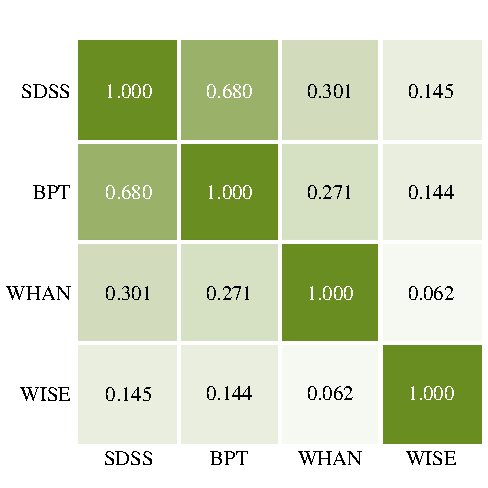
\includegraphics[width=\columnwidth, draft=false]{assets/plots/MCC_strict.pdf}
		\caption{}
		\label{fig:MCC_strict}
	\end{figure}

	\begin{figure}
		\centering
		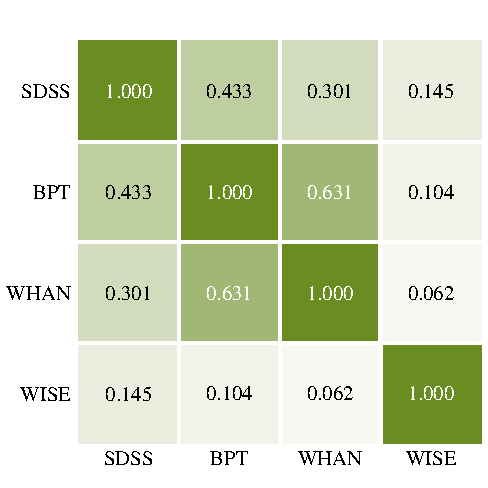
\includegraphics[width=\columnwidth, draft=false]{assets/plots/MCC_relaxed.pdf}
		\caption{}
		\label{fig:MCC_relaxed}
	\end{figure}

	\begin{figure}
		\centering
		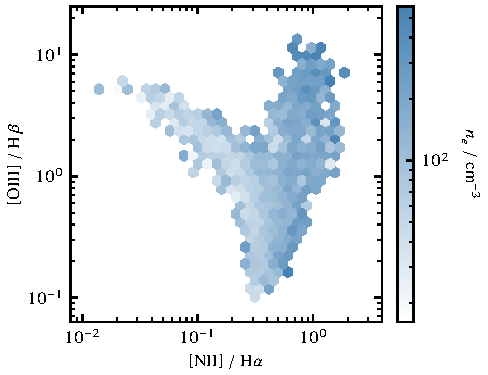
\includegraphics[width=\columnwidth, draft=false]{assets/plots/BPT_density.pdf}
		\caption{}
		\label{fig:BPT_density}
	\end{figure}

	\begin{figure}
		\centering
		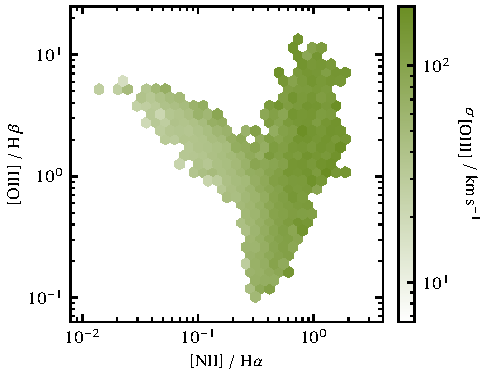
\includegraphics[width=\columnwidth, draft=false]{assets/plots/BPT_dispersion.pdf}
		\caption{}
		\label{fig:BPT_dispersion}
	\end{figure}

	\begin{figure}
		\centering
		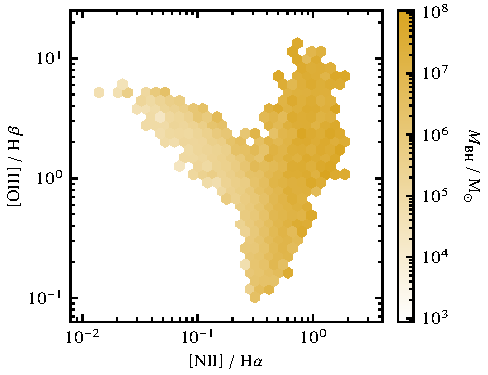
\includegraphics[width=\columnwidth, draft=false]{assets/plots/BPT_mass.pdf}
		\caption{}
		\label{fig:BPT_mass}
	\end{figure}

	\begin{figure}
		\centering
		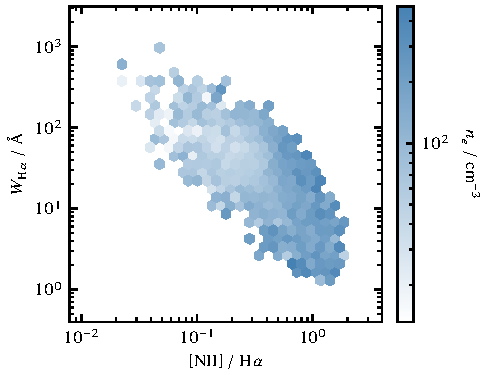
\includegraphics[width=\columnwidth, draft=false]{assets/plots/WHAN_density.pdf}
		\caption{}
		\label{fig:WHAN_density}
	\end{figure}

	\begin{figure}
		\centering
		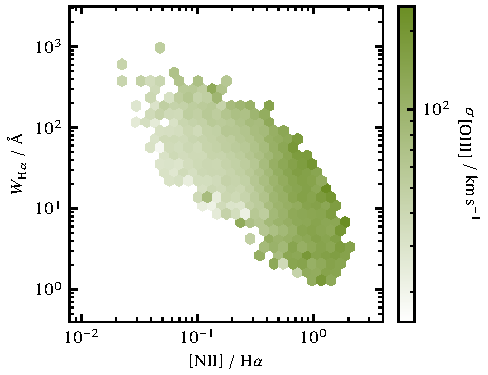
\includegraphics[width=\columnwidth, draft=false]{assets/plots/WHAN_dispersion.pdf}
		\caption{}
		\label{fig:WHAN_dispersion}
	\end{figure}

	\begin{figure}
		\centering
		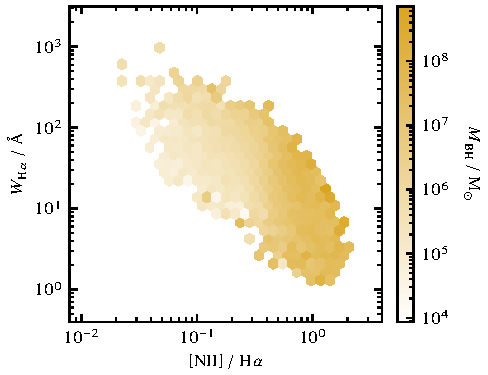
\includegraphics[width=\columnwidth, draft=false]{assets/plots/WHAN_mass.pdf}
		\caption{}
		\label{fig:WHAN_mass}
	\end{figure}

	\begin{figure}
		\centering
		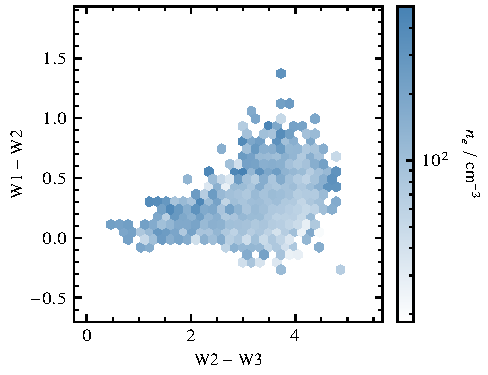
\includegraphics[width=\columnwidth, draft=false]{assets/plots/WISE_density.pdf}
		\caption{}
		\label{fig:WISE_density}
	\end{figure}

	\begin{figure}
		\centering
		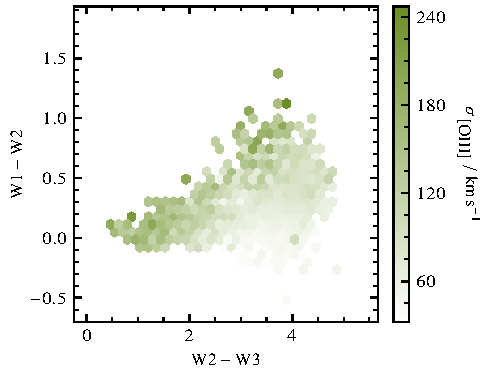
\includegraphics[width=\columnwidth, draft=false]{assets/plots/WISE_dispersion.pdf}
		\caption{}
		\label{fig:WISE_dispersion}
	\end{figure}

	\begin{figure}
		\centering
		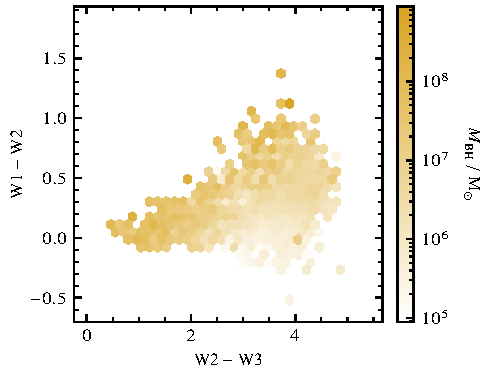
\includegraphics[width=\columnwidth, draft=false]{assets/plots/WISE_mass.pdf}
		\caption{}
		\label{fig:WISE_mass}
	\end{figure}

	\begin{figure*}[t]
		\centering
		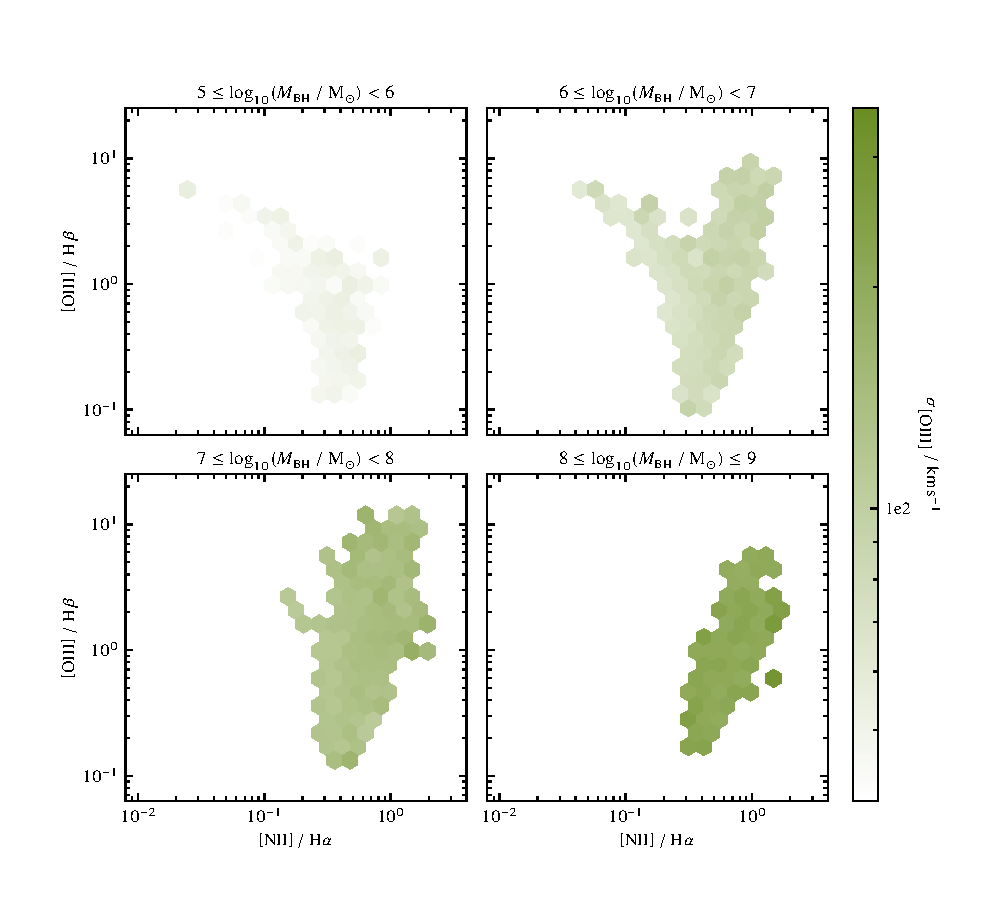
\includegraphics[width=\textwidth, draft=false]{assets/plots/BPT_bins.pdf}
		\caption{}
		\label{fig:BPT_bins}
	\end{figure*}

	\begin{figure*}[t]
		\centering
		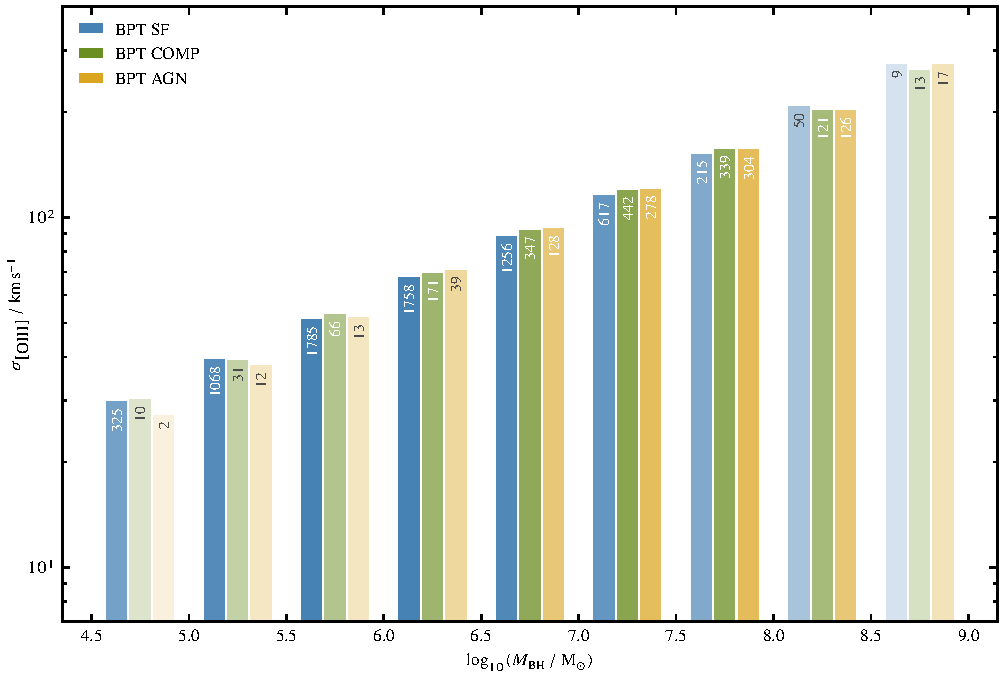
\includegraphics[width=\textwidth, draft=false]{assets/plots/BPT_bar.pdf}
		\caption{}
		\label{fig:BPT_bar}
	\end{figure*}

	\begin{figure*}[t]
		\centering
		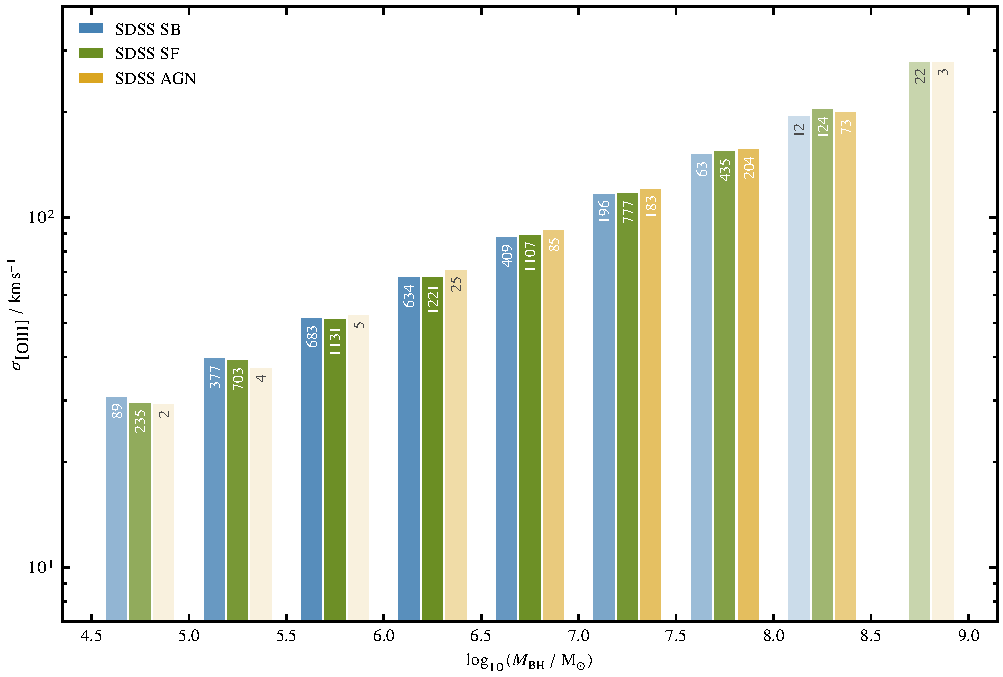
\includegraphics[width=\textwidth, draft=false]{assets/plots/SDSS_bar.pdf}
		\caption{}
		\label{fig:SDSS_bar}
	\end{figure*}

	\begin{figure*}[t]
		\centering
		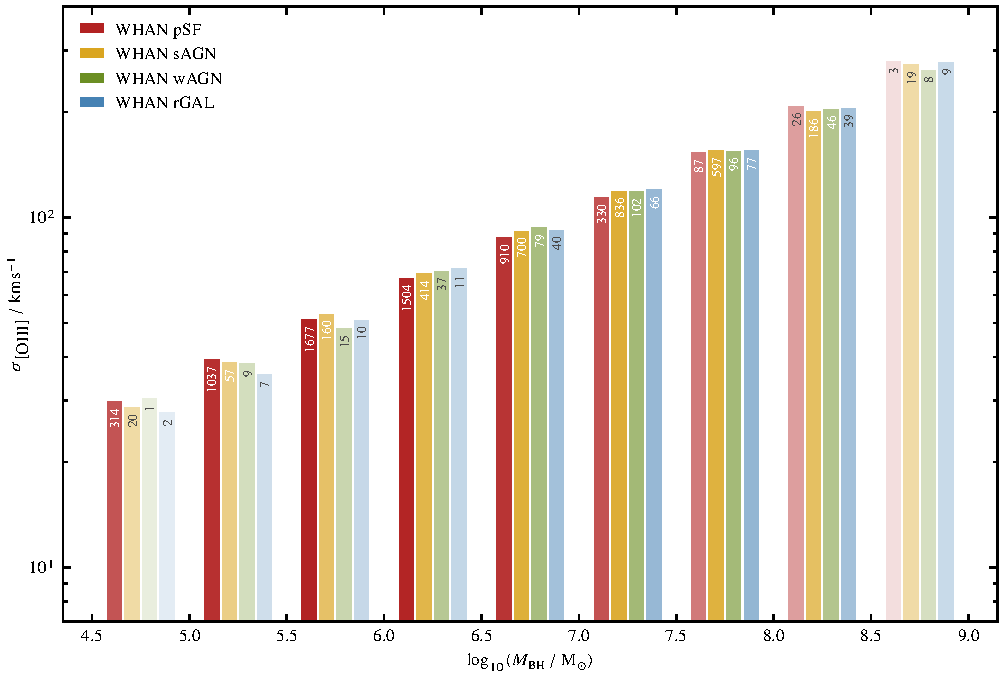
\includegraphics[width=\textwidth, draft=false]{assets/plots/WHAN_bar.pdf}
		\caption{}
		\label{fig:WHAN_bar}
	\end{figure*}

	\begin{figure*}[t]
		\centering
		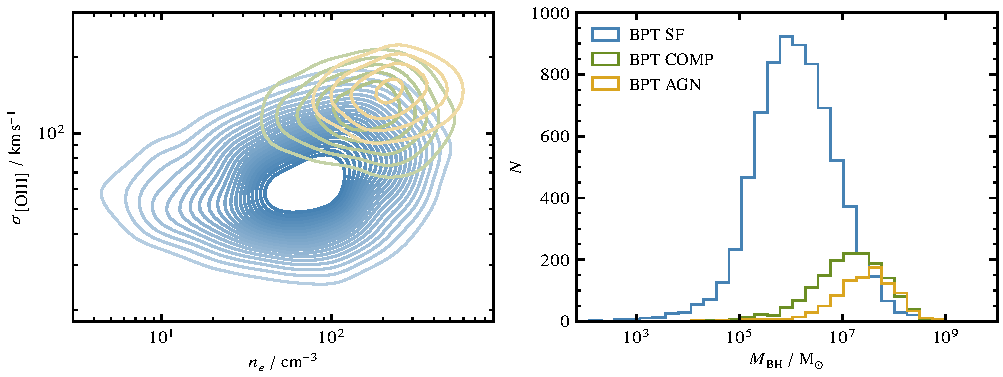
\includegraphics[width=\textwidth, draft=false]{assets/plots/BPT_multipanel.pdf}
		\caption{}
		\label{fig:BPT_multipanel}
	\end{figure*}

	\begin{figure*}[t]
		\centering
		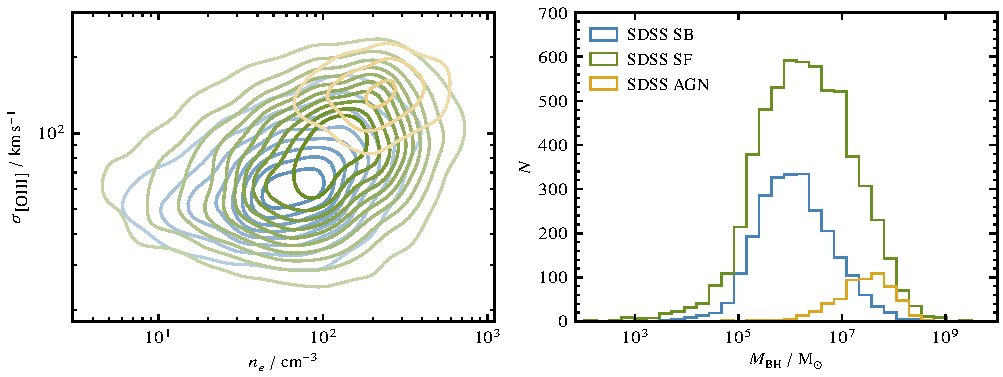
\includegraphics[width=\textwidth, draft=false]{assets/plots/SDSS_multipanel.pdf}
		\caption{}
		\label{fig:SDSS_multipanel}
	\end{figure*}

	\begin{figure*}[t]
		\centering
		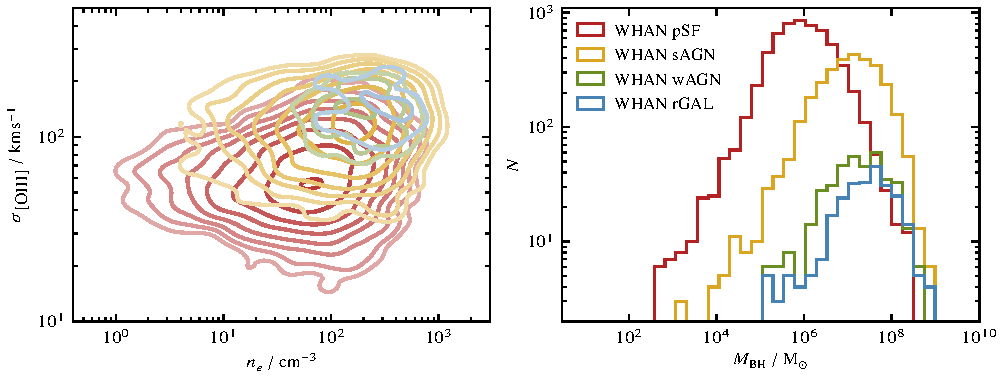
\includegraphics[width=\textwidth, draft=false]{assets/plots/WHAN_multipanel.pdf}
		\caption{}
		\label{fig:WHAN_multipanel}
	\end{figure*}

	

	\twocolumn[{\printbibliography\vspace{15\baselineskip}}]

	\pagenumbering{roman}
	\setcounter{page}{1}

	\section*{Appendix}
	\label{sec:appendix}

	\setcounter{subsection}{0}
	\renewcommand{\thesubsection}{\Alph{subsection}}

	\begin{figure*}[t]
	\centering
		\begin{center}
			\begin{varwidth}{0.875\textwidth}
\begin{lstlisting}
SELECT TOP 10000
    g.sii_6717_flux, g.sii_6731_flux, g.nii_6584_flux, g.oi_6300_flux, g.oiii_5007_flux,
    g.h_alpha_flux, g.h_beta_flux,
    g.h_alpha_eqw, g.nii_6584_eqw, g.oiii_sigma,
    w.w1mpro, w.w2mpro, w.w3mpro,
    s.z, s.class, s.subclass, s.bestobjid
FROM SpecObj AS s
    JOIN galSpecLine AS g ON s.specobjid = g.specobjid
    JOIN PhotoTag AS p ON s.bestobjid = p.objid
    OUTER APPLY (   SELECT TOP 1 x.wise_cntr
                    FROM wise_xmatch AS x
                    WHERE p.objid = x.sdss_objid AND x.match_dist < 3 
                    ORDER BY x.match_dist ASC
                ) AS y
    LEFT JOIN wise_allsky AS w ON y.wise_cntr = w.cntr
WHERE s.class = 'GALAXY'
    AND s.subclass != 'BROADLINE'
    AND s.subclass != 'AGN BROADLINE'
    AND s.subclass != 'STARFORMING BROADLINE'
    AND s.subclass != 'STARBURST BROADLINE'
    AND s.snmedian_r > 5.0
    AND s.z < 0.35
    AND g.sii_6717_eqw < 0.0
    AND g.sii_6731_eqw < 0.0
    AND g.nii_6584_eqw < 0.0
    AND g.oi_6300_eqw < 0.0
    AND g.oiii_5007_eqw < 0.0 
    AND g.h_alpha_eqw < 0.0
    AND g.h_beta_eqw < 0.0
    AND (2.355 * g.sigma_forbidden) < 500 
    AND (2.355 * g.sigma_balmer) < 500 
    AND g.sii_6717_flux > 3 * g.sii_6717_flux_err
    AND g.sii_6731_flux > 3 * g.sii_6731_flux_err
    AND g.nii_6584_flux > 3 * g.nii_6584_flux_err
    AND g.oi_6300_flux > 3 * g.oi_6300_flux_err
    AND g.oiii_5007_flux > 3 * g.oiii_5007_flux_err
    AND g.h_alpha_flux > 3 * g.h_alpha_flux_err
    AND g.h_beta_flux > 3 * g.h_beta_flux_err
ORDER BY s.specobjid ASC\end{lstlisting}
			\end{varwidth}
		\end{center}
	\end{figure*}

\end{document}

